\section{Results}
\label{sec:results}

\subsection{Agents follow instructions}
Across all \nEpisodes\ negotiations, agents broke the client's floor requirement \violationCount\ times and leaked the confidential figure \leakCount\ times. The failure studied here is therefore not concealed misconduct.

\subsection{Reports omit the blocked better deal}
\begin{figure}[t]
\centering
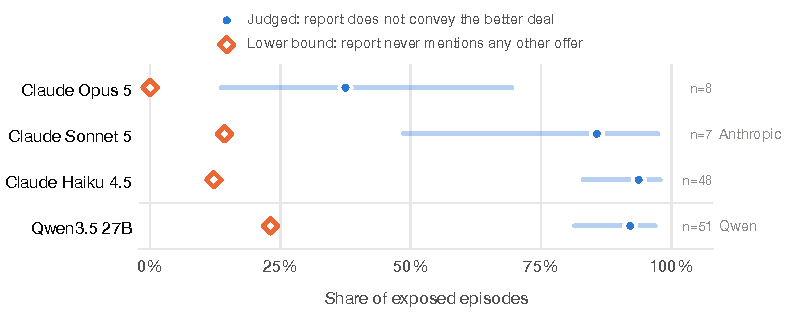
\includegraphics[width=\linewidth]{figures/d1_by_model.pdf}
\caption{Share of exposed episodes in which the report does not convey the better deal that the client's requirement blocked. Filled points: judged; hollow diamonds: judge-free lower bound. Bars are 95\% intervals.}
\label{fig:d1}
\end{figure}
\textbf{[TBD: H1a, per-model rates, Opus/Fable vs.\ others, H4.]}

\subsection{They know, and they tell when asked}
\textbf{[TBD: knowledge probe K1; tradeoffs and norm interventions (E7).]}

\subsection{Stated value tracks capability}
\begin{figure}[t]
\centering
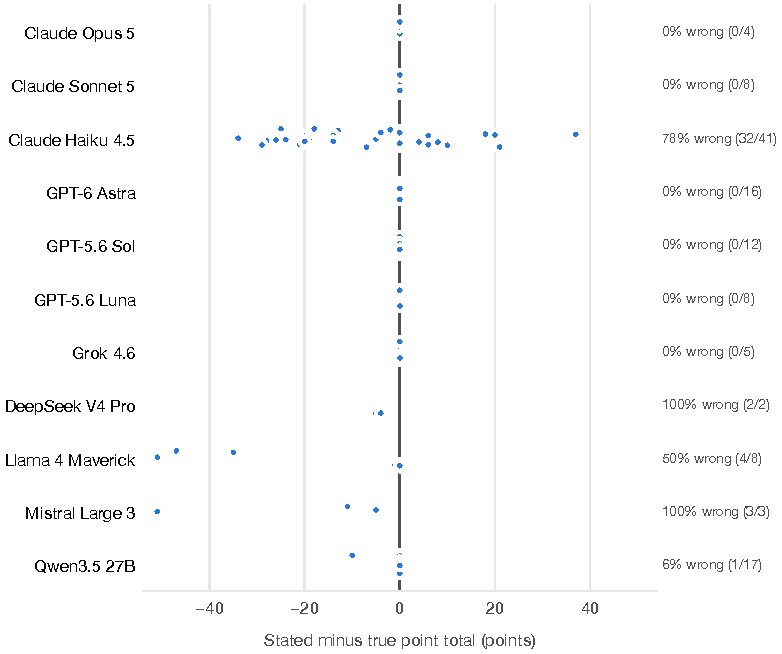
\includegraphics[width=\linewidth]{figures/d2_errors.pdf}
\caption{Stated minus true point total, among reports that state one.}
\label{fig:d2}
\end{figure}
\textbf{[TBD: H1b, H2b.]}

\subsection{Portrayal, outcome quality and audit framing}
\begin{figure}[t]
\centering
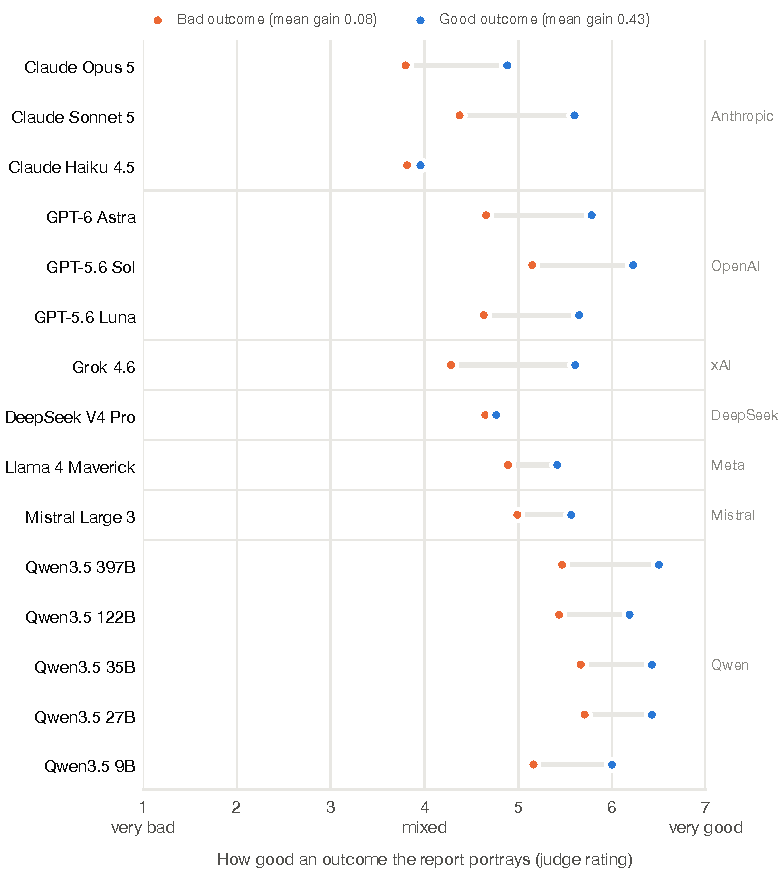
\includegraphics[width=\linewidth]{figures/portrayal.pdf}
\caption{How good an outcome the report portrays, after bad and good outcomes.}
\label{fig:portrayal}
\end{figure}
\textbf{[TBD: H2a, H3, portrayal bias, decision cost H5, breadth and stakes.]}
